\appendix

\chapter{Sward Learning Algorithm} \label{slalgo}
\section{Training Step} \label{slalgo:ul}
\begin{algorithm}[H]
	\caption{Training Step - Called Repeatedly in a Loop}
	\begin{algorithmic}[1]
		\State \Call{Train}{localModel, localData}
		\ForAll{$n \in neighbors$}
		\State \Call{SendTo}{$(localModel, localTrainingCounter)$, $n$}
		\EndFor
		
		\For{$x \in range(maxSyncWaits)$}
		\State $neighborModels \gets \emptyset$
		\ForAll{$n \in neighbors$}
		\State $model, traningCounter \gets$ \Call{CacheLookup}{$n$}
		\If{$trainingCounter + \beta \ge localTrainingCounter$}
		\State \Call{Append}{$neighborModels$, $model$}
		\EndIf
		\EndFor
		\If{$length_{neighborModels} \ge \gamma$}
		\If{$syncronisationMethod = "AVG"$}
		\State $localModel \gets \mu(localModel \cup neighborModels)$
		\ElsIf{$syncronisationMethod = "ASR"$}
		\State $localModel \gets (1 - \alpha) * localModel + \alpha * \mu(neighborModels)$
		\EndIf
		\Else
		\State continue
		\EndIf
		\State \Call{Sleep}{syncWaitTime}
		\EndFor
	\end{algorithmic}
\end{algorithm}

\section{Model Received Event} \label{slalgo:mre}
\begin{algorithm}[H]
	\caption{Model Received Event - Called When a Model Update is Received from a Remote Node}
	\textbf{Input}: $neighbour$, $nModel$, $nTrainingCounter$
	\newline
	\begin{algorithmic}[1]
		\If{\Call{InCache}{$neighbour$}}
			\State $\_, nTraningCounterOld \gets$ \Call{CacheLookup}{$n$}
			\If{$nTrainingCounter > nTraningCounterOld$}
				\State \Call{SetCache}{$neighbour$, $(nModel, nTrainingCounter)$}
			\EndIf
		\Else
			\State \Call{SetCache}{$neighbour$, $(nModel, nTrainingCounter)$}
		\EndIf
	\end{algorithmic}
\end{algorithm}


\chapter{Machine Learning Model} \label{ap:model}
\begin{lstlisting}[language=Python]
inp = Input((28,28))
out = Reshape((28,28,1))(inp)
out = Conv2D(16, (3,3), activation="relu")(out)
out = Conv2D(16, (3,3), activation="relu")(out)
out = Flatten()(out)
out = Dense(256, activation="relu")(out)
out = Dense(128, activation="relu")(out)
out = Dense(10, activation="sigmoid")(out)
model = Model(inputs=inp, outputs=out)
model.compile(
	optimizer="adam",
	loss=SparseCategoricalCrossentropy(),
	metrics=[SparseCategoricalAccuracy()]
)
\end{lstlisting}

\chapter{Gantt Charts}
\newpage
\section{Gantt - Interim} \label{gc-interim}
\begin{center}
	\rotatebox[origin=c]{-90}{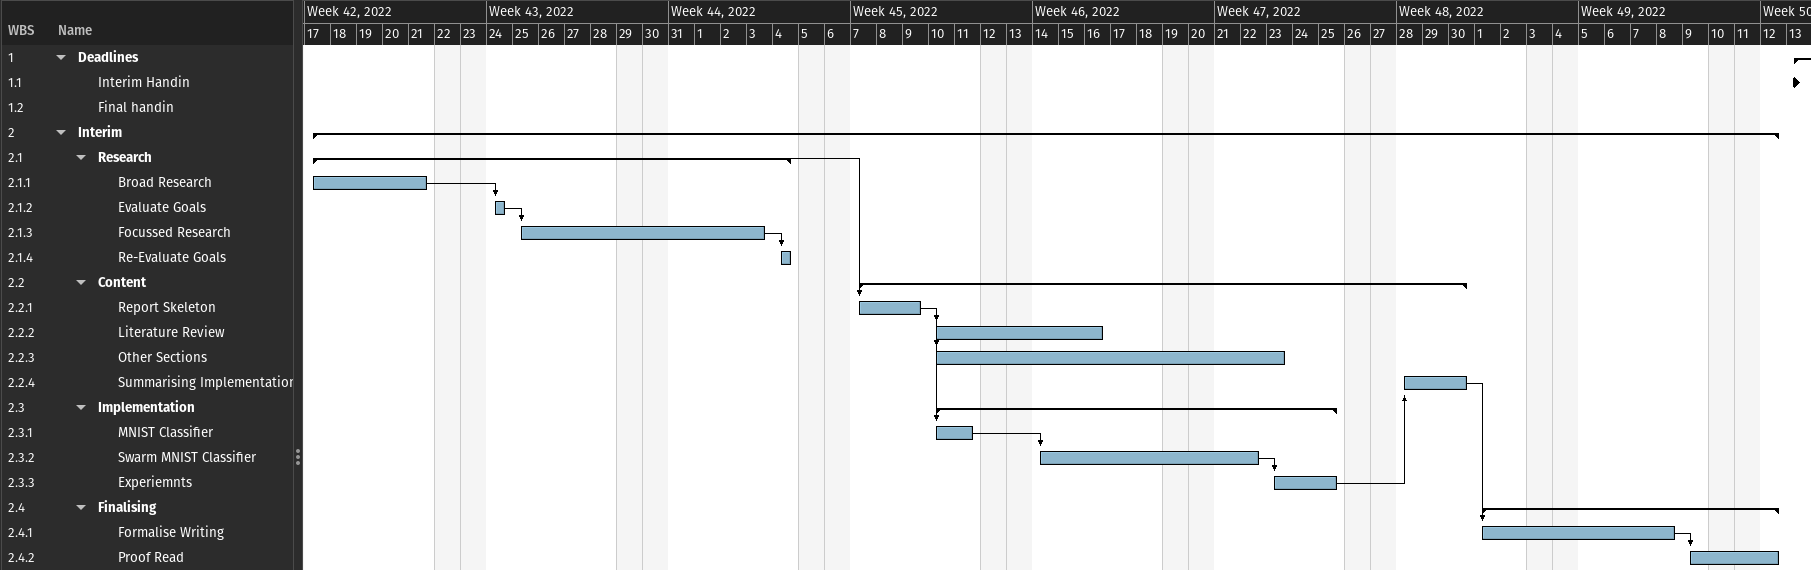
\includegraphics[width=\textheight]{gannt-interim}}
\end{center}

\section{Gantt - Final} \label{gc-final}
\begin{center}
	\rotatebox[origin=c]{-90}{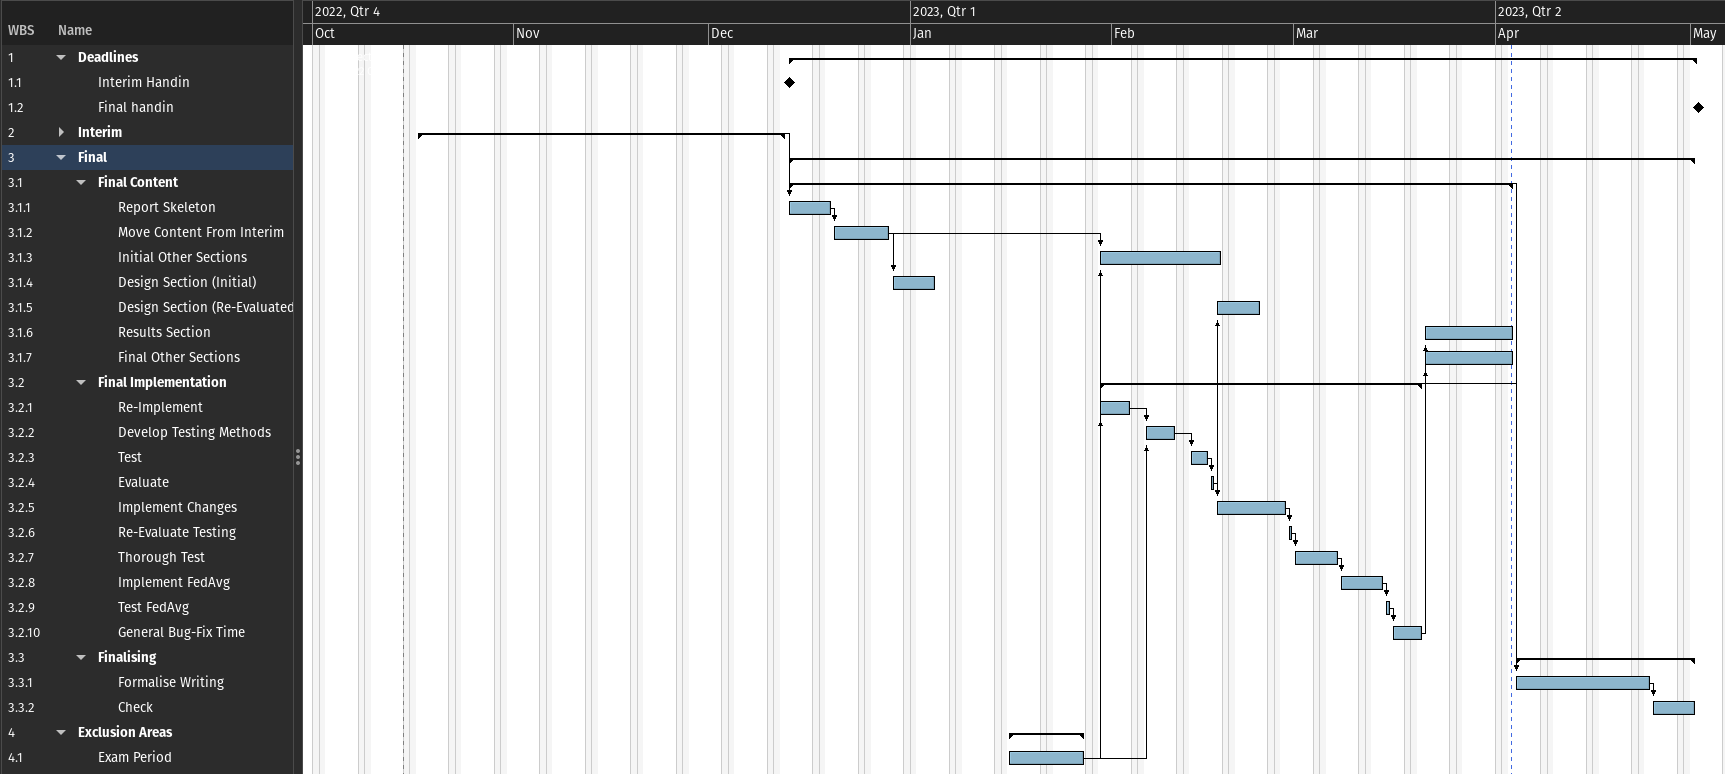
\includegraphics[width=\textheight]{gannt-final}}
\end{center}